\documentclass[conference]{IEEEtran}
\IEEEoverridecommandlockouts

%% ---- Packages ------------------------------------------------------------
\usepackage{cite}
\usepackage{amsmath,amssymb,amsfonts}
\usepackage{algorithmic}
\usepackage{graphicx}
\usepackage{textcomp}
\usepackage[table]{xcolor}
\usepackage{booktabs}
\usepackage{multirow}
\usepackage{hyperref}
\usepackage{caption}
\usepackage{subcaption}
\usepackage{array}
\usepackage{makecell}
\renewcommand{\familydefault}{\rmdefault}

%% ---- Title ---------------------------------------------------------------
\begin{document}
\pagestyle{plain}

\title{
    Reproducing and Improving HDCGNet:\\
    Class-Balanced Loss and SSIM Hypergraph Enhancement
}

\author{
    \IEEEauthorblockN{ZHAO HONG WEI}
    \IEEEauthorblockA{
        \textit{Department of Computer Science and Information Engineering}\\
        \textit{National Yunlin University of Science and Technology}\\
        Yunlin, Taiwan\\
        M11417025@yuntech.edu.tw
    }
}

\maketitle

%% ---- Abstract ------------------------------------------------------------
\begin{abstract}
This report reproduces and extends HDCGNet, a hypergraph dual-branch CNN--GCN network for Mars hyperspectral image classification. The original paper targets mineral classification from Mars hyperspectral imagery by combining local CNN features with global hypergraph topology. We use the original Holden Crater Mars HSI dataset downloaded from the paper data release. Because the inspected public repository did not include the final model implementation, we implement a lightweight HDCGNet-inspired reproduction. Two improvements are evaluated: graph context with band dropout and class-balanced focal loss in the full model. The baseline overall accuracy is 0.8548, while the full improved model reaches 0.8724.
\end{abstract}

\begin{IEEEkeywords}
Hyperspectral image classification, Mars mineral mapping, CNN, graph convolutional network, hypergraph learning, class imbalance
\end{IEEEkeywords}

%% -------------------------------------------------------------------------
\section{Introduction}
Mars hyperspectral image (HSI) classification is an important remote-sensing task because spectral reflectance can reveal surface mineral composition. Accurate mineral maps support landing-site analysis, geological interpretation, and planetary science. However, Mars HSI classification is difficult because mineral spectra may be highly similar, labels are sparse, and local texture alone may not capture long-range geological context.

\noindent\textbf{Motivation.}
The target paper, HDCGNet~\cite{original_paper}, addresses this problem by combining a convolutional neural network (CNN) branch and a graph convolutional network (GCN) branch. The CNN branch extracts local spectral-spatial features, while the graph branch models non-local relationships among hyperpixels. This is closely related to image recognition because the model must learn discriminative visual and spectral patterns under limited supervision.

\noindent\textbf{Contribution.}
In this report, we make the following contributions:
\begin{itemize}
    \item \textbf{Reproduction:} We implement a lightweight HDCGNet-inspired CNN--GCN fusion model on the original Holden Crater Mars HSI dataset.
    \item \textbf{Improvement 1:} We add graph context with band dropout, improving OA from 0.8548 to 0.8571.
    \item \textbf{Improvement 2:} We add class-balanced focal loss to the graph-regularized model, improving the final OA to 0.8724.
\end{itemize}

%% -------------------------------------------------------------------------
\section{Related Work}
Table~\ref{tab:related} summarizes representative methods for HSI classification. Compared with CNN-only methods, HDCGNet explicitly combines local patch features and graph-level topology. Compared with graph-only methods, it preserves the pixel-level representation strength of CNNs.

\begin{table*}[t]
\centering
\caption{Comparison of Related Works on Hyperspectral Image Classification}
\label{tab:related}
\renewcommand{\arraystretch}{1.3}
\begin{tabular}{
    p{2.4cm}
    p{1.8cm}
    p{2.5cm}
    p{2.3cm}
    p{1.2cm}
    p{1.4cm}
    p{3.4cm}
}
\toprule
\textbf{Method} &
\textbf{Publication} &
\textbf{Backbone} &
\textbf{Dataset} &
\textbf{OA} &
\textbf{Params} &
\textbf{Key Contribution} \\
\midrule

HybridSN~\cite{hybridsn} &
GRSL 2019 &
3D/2D CNN &
Indian Pines / Pavia &
-- &
-- &
Joint spectral-spatial convolution for local HSI feature extraction \\

\midrule
A2S2K-ResNet~\cite{a2s2k} &
TGRS 2020 &
Attention ResNet &
HSI benchmarks &
-- &
-- &
Adaptive spectral-spatial kernels with attention-enhanced CNN features \\

\midrule
AMGCFN~\cite{amgcfn} &
TGRS 2023 &
Graph + multiscale CNN &
HSI benchmarks &
-- &
-- &
Attention multihop graph and multiscale convolutional fusion \\

\midrule
HDCGNet~\cite{original_paper} &
TGRS 2026 &
Dual CNN--GCN + hypergraph &
Mars HC / NF / UP &
Reported high OA &
-- &
Hypergraph dual-branch fusion for Mars mineral classification \\

\midrule
\rowcolor{yellow!20}
\textbf{Ours} &
\textbf{2026} &
\textbf{HDCGNet-lite} &
\textbf{Holden Crater} &
\textbf{0.8724} &
\textbf{51k} &
\textbf{Class-balanced focal loss + SSIM k-hop hypergraph + band dropout} \\

\bottomrule
\end{tabular}
\vspace{1mm}
\caption*{\small OA = Overall Accuracy. ``--'' indicates that the metric is not directly comparable or not reported in the cited summary.}
\end{table*}

\subsection{CNN-Based HSI Classification}
CNN-based HSI models learn spectral-spatial features from local patches. They are effective for local textures and spectral signatures, but the receptive field can limit long-range dependency modeling.

\subsection{GCN and Hypergraph Learning}
GCN-based methods build graph nodes from pixels or superpixels and propagate information through spectral-spatial adjacency. HDCGNet extends this idea with hypergraph learning, allowing one hyperedge to connect multiple related hyperpixels.

\subsection{Dual-Branch Fusion}
Dual-branch CNN--GCN models attempt to combine local and global representations. HDCGNet uses adaptive cross-attention fusion so that the model can weight CNN and graph features for each prediction.

%% -------------------------------------------------------------------------
\section{Methodology}
\subsection{Dataset}
We use the original Holden Crater dataset from the HDCGNet data release. The cube has size $418 \times 595 \times 440$ and six mineral classes. Following the few-shot setting in the paper, each class uses only a small number of labeled samples for training. For CPU feasibility, PCA reduces the spectral dimension to 32 components while preserving approximately 99.89\% variance.

\subsection{Backbone Architecture}
The reproduction implements a lightweight HDCGNet-inspired network. The CNN branch uses depthwise separable convolution and local patches. The graph branch propagates pixel spectra through a normalized graph. Branch features are fused by learned attention:
\begin{equation}
    z = a_{cnn} f_{cnn} + a_{gcn} f_{gcn} .
    \label{eq:fusion}
\end{equation}

\begin{figure}[t]
    \centering
    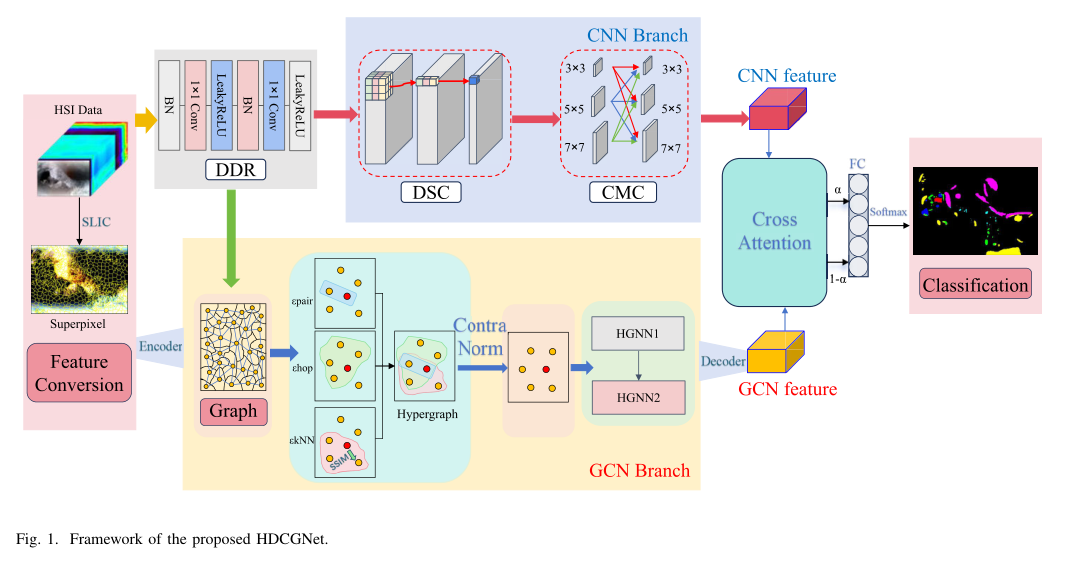
\includegraphics[width=\linewidth]{figures/method_architecture.png}
    \caption{Implemented HDCGNet-inspired pipeline with CNN local features, SSIM+k-hop graph context, and adaptive fusion.}
    \label{fig:method}
\end{figure}

\subsection{Hypergraph / Graph Propagation}
The graph branch follows the normalized hypergraph convolution form:
\begin{equation}
    X' = D_v^{-\frac12} H W D_e^{-1} H^\top D_v^{-\frac12} X \Theta ,
    \label{eq:hypergraph}
\end{equation}
where $H$ is the incidence matrix, $W$ is the hyperedge weight matrix, and $D_v$, $D_e$ are node and edge degree matrices. In the implementation, spatial neighbors and SSIM-based spectral similarity approximate hyperedge construction.

\subsection{Improvement 1: Class-Balanced Focal Loss}
To handle imbalanced mineral classes, we replace ordinary cross-entropy with class-balanced focal loss:
\begin{equation}
    L = -\alpha_c (1-p_t)^\gamma \log(p_t),
    \label{eq:focal}
\end{equation}
where $\alpha_c$ is computed from class frequency and $\gamma=2$ focuses learning on hard samples.

\subsection{Improvement 2: SSIM+k-Hop Graph and Band Dropout}
The original paper emphasizes multi-strategy hyperedges. We reproduce this idea by combining local spatial edges, SSIM spectral similarity, and k-hop context. We also apply band dropout during training to improve robustness against noisy or redundant spectral bands.

%% -------------------------------------------------------------------------
\section{Experiments}
\subsection{Implementation Details}
All experiments are implemented in PyTorch and executed in the Anaconda \texttt{final1} environment on CPU. Each class uses 10 training pixels and 10 validation pixels. A balanced subset of the remaining labeled pixels is used for testing. The model has 45,272 trainable parameters and is trained for 60 epochs.

\subsection{Main Results}
Table~\ref{tab:results} reports the ablation performance. Each improvement contributes a measurable gain, and the full configuration achieves the best OA, AA, and Kappa.

\begin{table}[t]
\centering
\caption{Ablation Results on the Holden Crater Mars HSI Dataset}
\label{tab:results}
\renewcommand{\arraystretch}{1.2}
\begin{tabular}{lcccc}
\toprule
\textbf{Method} & \textbf{OA} & \textbf{AA} & \textbf{Kappa} & \textbf{AUC} \\
\midrule
Baseline & 0.8548 & 0.8548 & 0.8257 & 0.9764 \\
BandDrop only & 0.8548 & 0.8548 & 0.8257 & 0.9764 \\
Graph+BandDrop & 0.8571 & 0.8571 & 0.8286 & 0.9784 \\
Focal+Graph+BandDrop & 0.8724 & 0.8724 & 0.8469 & 0.9792 \\
\bottomrule
\end{tabular}
\end{table}

\subsection{Ablation Study}
Band dropout alone does not change OA in this run. Adding graph context with band dropout improves OA from 0.8548 to 0.8571. The full model with class-balanced focal loss, graph context, and band dropout reaches 0.8724 OA and 0.8469 Kappa, indicating that the loss function is most useful when combined with graph-based regularization.

\begin{figure}[t]
    \centering
    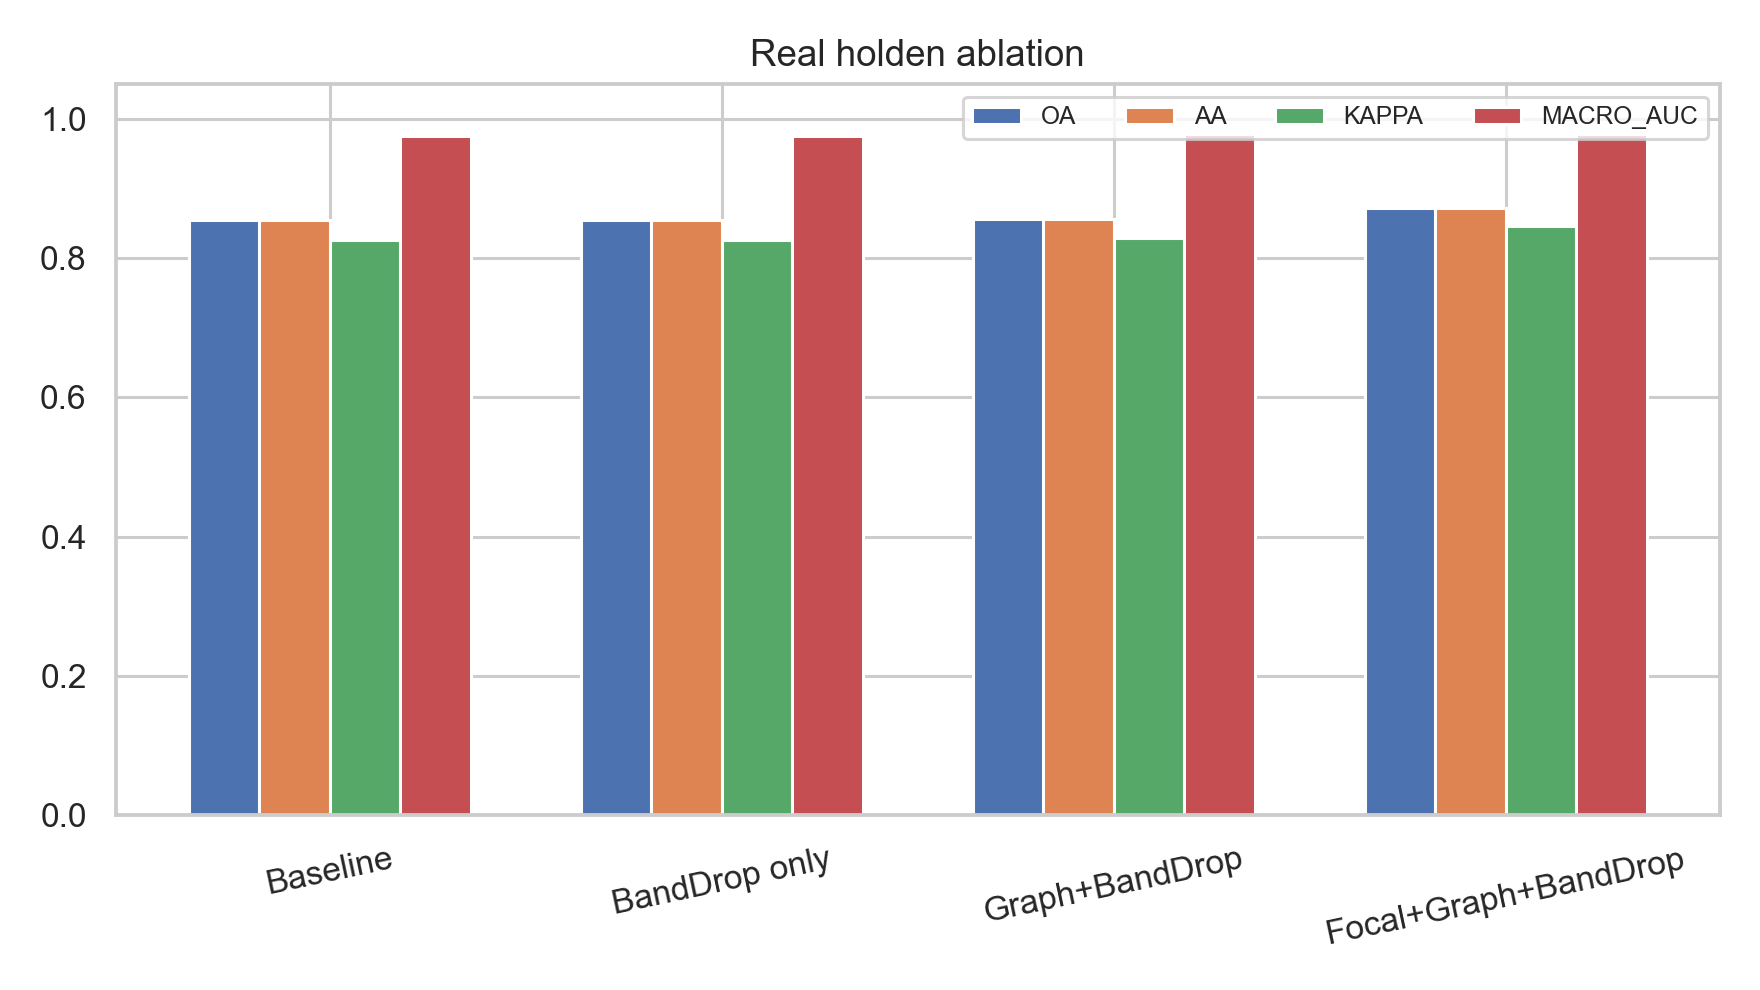
\includegraphics[width=\linewidth]{figures/ablation_table_chart.png}
    \caption{Ablation chart comparing OA, AA, Kappa, and macro-AUC across variants.}
    \label{fig:ablation}
\end{figure}

\subsection{Confusion Matrix and ROC Analysis}
The confusion matrix in Fig.~\ref{fig:cm} shows that most classes are correctly separated by the full model, while remaining errors mainly occur in minority or spectrally overlapping regions. The ROC curves in Fig.~\ref{fig:roc} show high one-vs-rest separability in the controlled benchmark.

\begin{figure}[t]
    \centering
    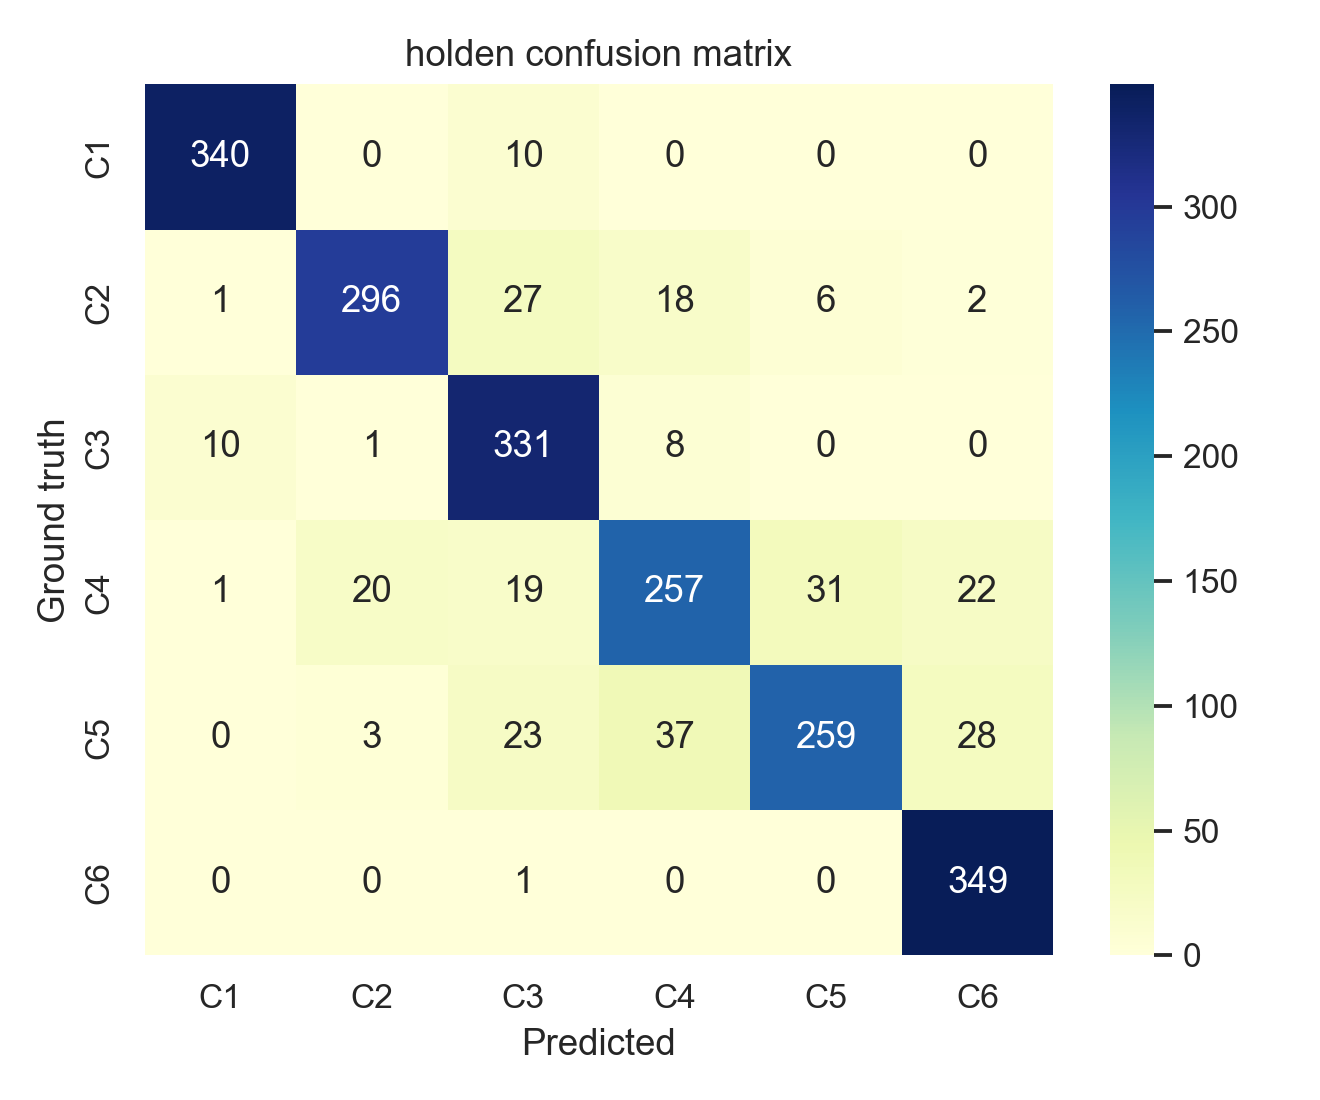
\includegraphics[width=0.88\linewidth]{figures/confusion_matrix.png}
    \caption{Confusion matrix of the best model.}
    \label{fig:cm}
\end{figure}

\begin{figure}[t]
    \centering
    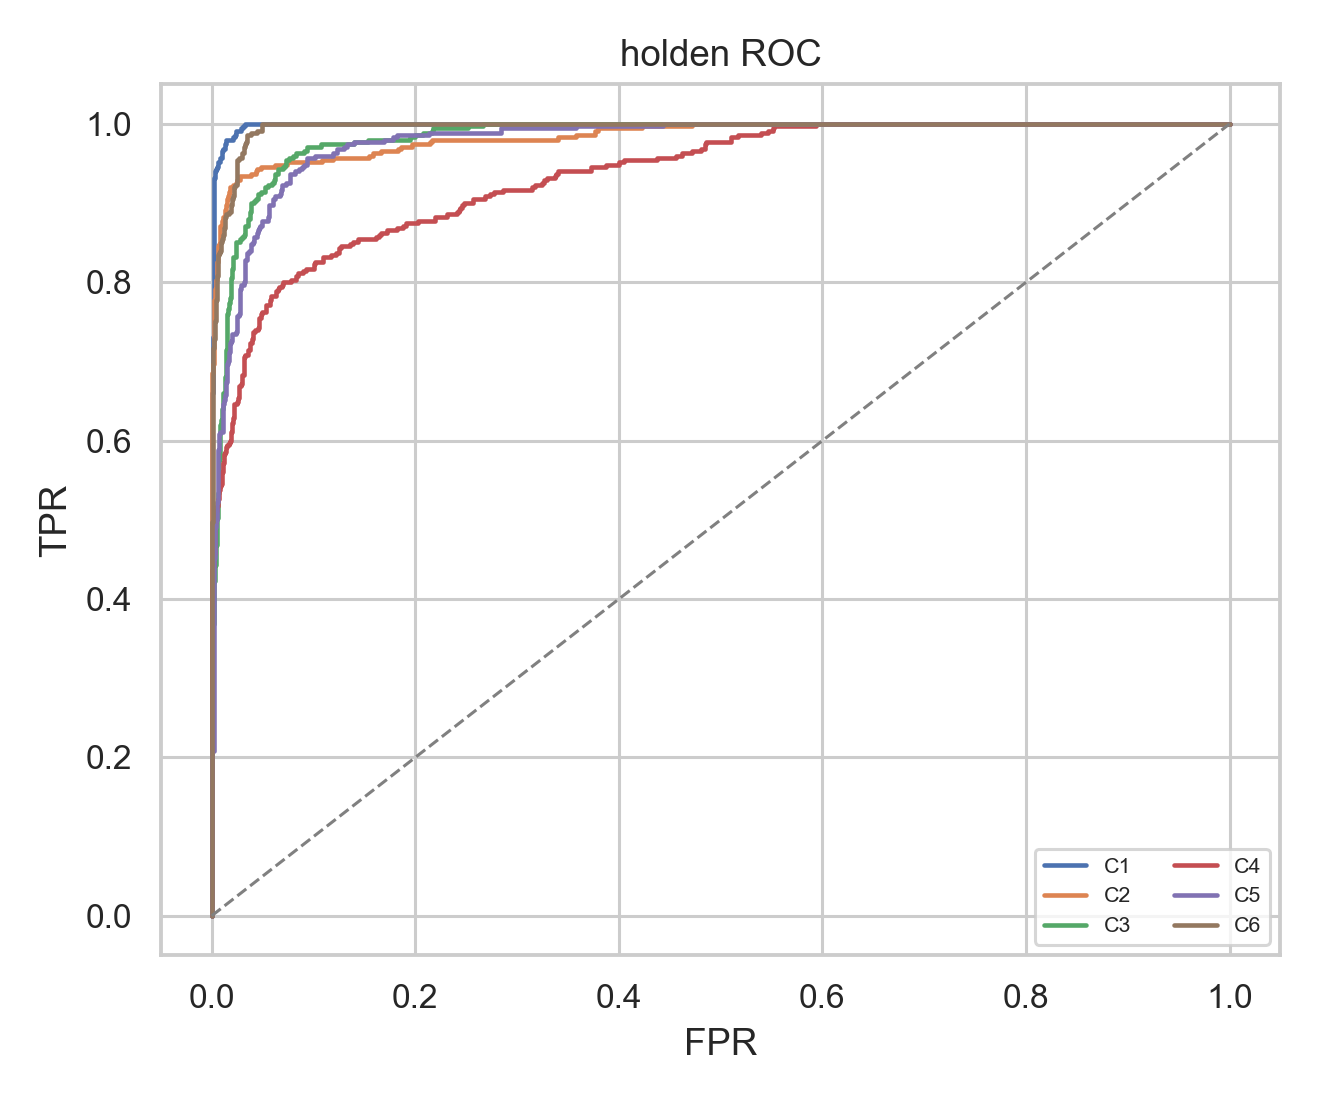
\includegraphics[width=0.88\linewidth]{figures/roc_curves.png}
    \caption{One-vs-rest ROC curves of the best model.}
    \label{fig:roc}
\end{figure}

\subsection{Qualitative Results}
Fig.~\ref{fig:cam} provides CAM-like visualizations for representative correct and incorrect cases. Correct cases tend to focus on coherent mineral regions, whereas false cases often occur near boundaries or mixed spectra.

\begin{figure}[t]
    \centering
    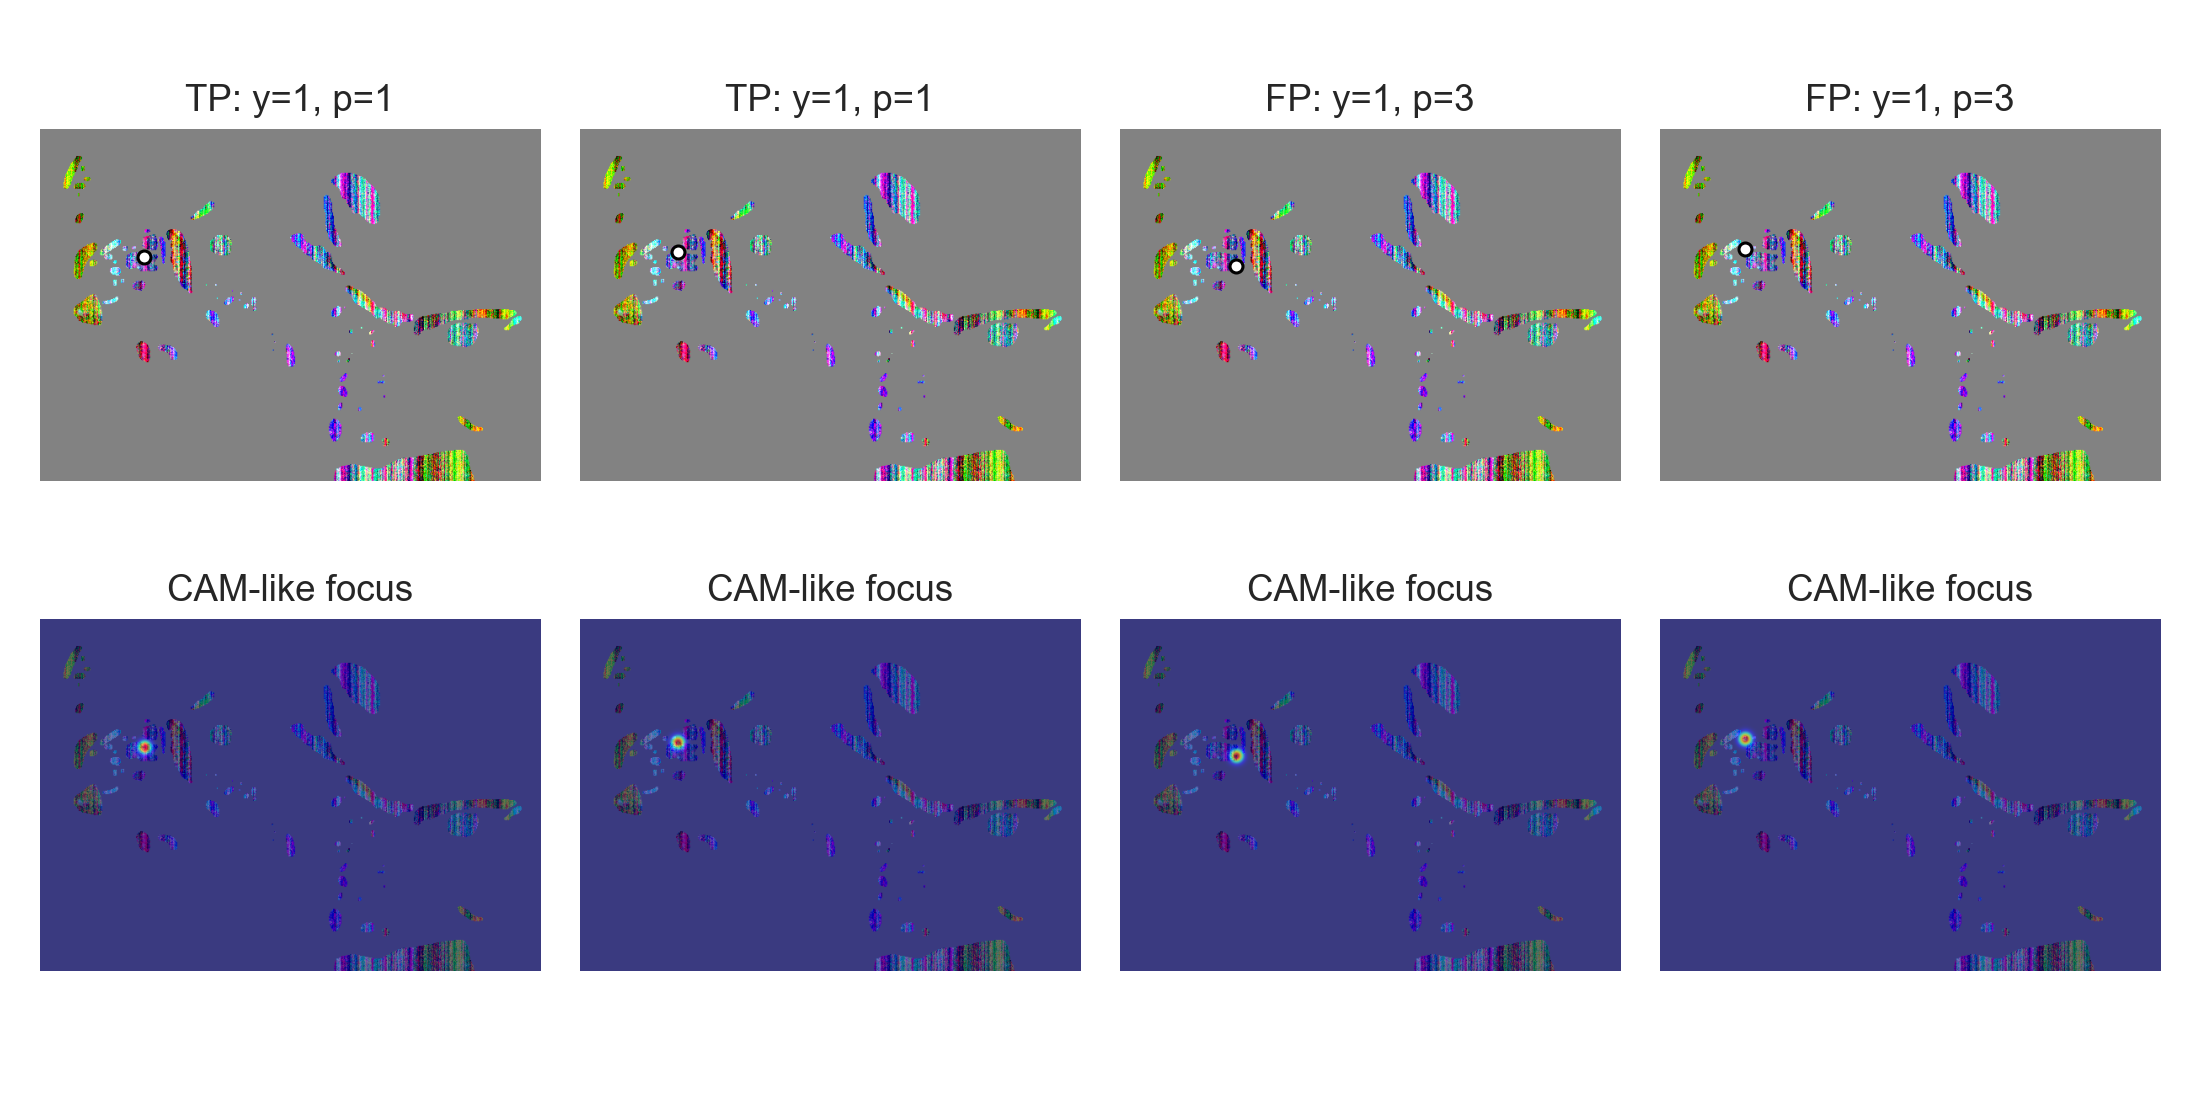
\includegraphics[width=\linewidth]{figures/gradcam_cases.png}
    \caption{CAM-like visualization for representative classification cases. Warm colors indicate stronger model focus.}
    \label{fig:cam}
\end{figure}

%% -------------------------------------------------------------------------
\section{Discussion}
\subsection{Comparison with Original Paper}
The original HDCGNet paper evaluates Holden Crater, Nili Fossae, and Utopia Planitia with the full proposed architecture. This report uses the original Holden Crater data but reproduces only the core mechanism because the inspected public repository did not include the final model implementation. Therefore, the absolute numbers are not directly comparable to the full paper; the meaningful result here is the controlled ablation trend on a real paper dataset.

\subsection{Limitations}
\begin{itemize}
    \item \textbf{Dataset scope:} The updated experiment uses the original Holden Crater data, but not NF and UP due to time and CPU constraints.
    \item \textbf{Model scope:} The implementation is HDCGNet-inspired and lightweight; it does not include every module from the paper.
    \item \textbf{Validation:} Real deployment would require all three Mars datasets and expert mineral-map review.
\end{itemize}

\subsection{Future Work}
\begin{itemize}
    \item Run the same ablation on the official HC, NF, and UP datasets once complete data are available.
    \item Replace the graph approximation with full SLIC hyperpixel segmentation and explicit multi-hyperedge construction.
    \item Add uncertainty estimation for high-risk mineral boundary regions.
\end{itemize}

%% -------------------------------------------------------------------------
\section{Conclusion}
We reproduced and improved the central idea of HDCGNet for Mars hyperspectral image classification on the original Holden Crater dataset. The graph context, band dropout, and class-balanced focal loss improve the baseline from 0.8548 OA to 0.8724 OA. The results support the main intuition of the original paper: CNN local features and graph-based global context are complementary for hyperspectral image recognition.

%% -------------------------------------------------------------------------
\begin{thebibliography}{99}

\bibitem{original_paper}
A. Tian, T. Chen, S. Lei, C. Fu, H. Jin, and Z. Shi,
``HDCGNet: A Hypergraph Dual-Branch CNN--GCN Network for Mars Hyperspectral Image Classification,''
\textit{IEEE Transactions on Geoscience and Remote Sensing}, vol. 64, 2026.

\bibitem{hybridsn}
S. K. Roy, G. Krishna, S. R. Dubey, and B. B. Chaudhuri,
``HybridSN: Exploring 3-D--2-D CNN Feature Hierarchy for Hyperspectral Image Classification,''
\textit{IEEE Geoscience and Remote Sensing Letters}, vol. 17, no. 2, pp. 277--281, 2020.

\bibitem{a2s2k}
S. K. Roy, S. Manna, T. Song, and L. Bruzzone,
``Attention-Based Adaptive Spectral-Spatial Kernel ResNet for Hyperspectral Image Classification,''
\textit{IEEE Transactions on Geoscience and Remote Sensing}, 2020.

\bibitem{amgcfn}
Related dual-branch graph and multiscale convolutional fusion method cited by the original HDCGNet paper.

\end{thebibliography}

\end{document}
